\documentclass{article}

\PassOptionsToPackage{numbers, sort, compress}{natbib}
\usepackage[main,preprint]{neurips_2025}

\usepackage[T1]{fontenc}
\usepackage[utf8]{inputenc}
\usepackage{hyperref}
\hypersetup{
  hidelinks,
  pdftitle={Adapting Activation-Aware Vector Quantization to Diffusion Transformers},
  pdfauthor={Egor Podyablonskiy and Aibek Alanov}
}
\usepackage{url}
\urlstyle{same}
\usepackage{booktabs}
\usepackage{nicefrac}
\usepackage{microtype}
\usepackage{xcolor}

%%%

\usepackage{subcaption}
\usepackage{graphicx}
\usepackage{multirow}
\usepackage{amsmath,amssymb,amsfonts}
\usepackage{amsthm}
\usepackage{mathrsfs}
\usepackage{xcolor}
\usepackage{textcomp}
\usepackage{manyfoot}
\usepackage{algorithm}
\usepackage{algorithmicx}
\usepackage{algpseudocode}
\usepackage{listings}

\newtheorem{theorem}{Theorem} % continuous numbers
%%\newtheorem{theorem}{Theorem}[section] % sectionwise numbers
%% optional argument [theorem] produces theorem numbering sequence instead of independent numbers for Proposition
\newtheorem{proposition}[theorem]{Proposition}%
\newtheorem{lemma}{Lemma}%
%%\newtheorem{proposition}{Proposition} % to get separate numbers for theorem and proposition etc.

\newtheorem{example}{Example}
\newtheorem{remark}{Remark}

\newtheorem{definition}{Definition}
\newtheorem{assumption}{Assumption}

%%%


\title{Adapting Activation-Aware Vector Quantization\\
to Diffusion Transformers}


% The \author macro works with any number of authors. There are two commands
% used to separate the names and addresses of multiple authors: \And and \AND.
%
% Using \And between authors leaves it to LaTeX to determine where to break the
% lines. Using \AND forces a line break at that point. So, if LaTeX puts 3 of 4
% authors names on the first line, and the last on the second line, try using
% \AND instead of \And before the third author name.


\author{
  Egor Podyablonskiy\\
  Lomonosov Moscow State University\\
  Faculty of Computational Mathematics and Cybernetics\\
  Moscow, Russia\\
  \And
  Aibek Alanov\\
  Scientific advisor\\
  Candidate of Physical and Mathematical Sciences\\
  Lomonosov Moscow State University\\
  Moscow, Russia\\
}


\begin{document}
\raggedbottom

\newcommand{\VQBits}{4.150}
\newcommand{\OriginalFID}{6.192}
\newcommand{\VQFID}{15.726}
\newcommand{\FIDGap}{9.534}
\newcommand{\VQSeconds}{5369.657}
\newcommand{\CalibrationSeconds}{1727.686}
\newcommand{\MiddleGainThousand}{37.03}
\newcommand{\MiddleLargeCILow}{34.49}
\newcommand{\MiddleLargeCIHigh}{39.53}
\newcommand{\AdaLNGainThousand}{30.80}
\newcommand{\FamilyBaseline}{0.125554}
\newcommand{\MiddleGainSmall}{36.49}
\newcommand{\MiddleCILow}{31.11}
\newcommand{\MiddleCIHigh}{41.91}
\newcommand{\LateGainSmall}{1.09}
\newcommand{\GateMLPGain}{10.41}
\newcommand{\GateMLPCILow}{7.01}
\newcommand{\GateMLPCIHigh}{13.73}
\newcommand{\ShiftMLPGain}{6.56}
\newcommand{\ShiftMLPCILow}{2.62}
\newcommand{\ShiftMLPCIHigh}{10.18}
\newcommand{\BaselineRows}{%
Original & 32.000 & 6.192 & 21.971 & 250.782 & 0.7848 & 0.6554 \\
VQDM transfer & 4.150 & 15.726 & 27.929 & 144.793 & 0.6372 & 0.7142 \\
}
\newcommand{\LiteratureRows}{%
VQ4DiT~\citep{deng2024vq4dit} & W3 & 6.72 & 11.91 & +5.19 & 24.18 \\
PTQ4DiT~\citep{wu2024ptq4dit} & W4A8 & 6.02 & 9.17 & +3.15 & 24.29 \\
HTG~\citep{ding2025htg} & W4A8 & 6.02 & 8.77 & +2.75 & 22.31 \\
}
\newcommand{\FamilyRows}{%
adaLN & 223.0 & 33.33\% & 0.086888 & 30.80\% \\
Attention & 148.6 & 22.22\% & 0.110884 & 11.68\% \\
MLP & 297.3 & 44.44\% & 0.104628 & 16.67\% \\
}
\newcommand{\WeightedRows}{%
Before refitting & 4.1501 & 15.726 & 27.929 & 144.799 & 0 \\
Uniform & 4.1501 & 15.604 & 27.858 & 145.739 & 200 \\
Last ten steps weighted $2\times$ & 4.1501 & 15.667 & 27.899 & 145.114 & 200 \\
Last twenty steps weighted $2\times$ & 4.1501 & 15.686 & 27.927 & 145.288 & 200 \\
}
\newcommand{\TemporalRows}{%
Before refitting & 4.1501 & 15.726 & 27.929 & 144.794 & 0 \\
Three temporal codebook sets & 4.2044 & 15.663 & 27.823 & 146.031 & 600 \\
One uniform codebook set & 4.1501 & 15.536 & 27.796 & 146.436 & 600 \\
}


\maketitle

\begin{abstract}
We study activation-aware vector quantization of DiT-XL/2. Transferred VQDM achieves \VQBits{} bits per parameter but raises ImageNet256 FID from \OriginalFID{} to \VQFID{}. Paired interventions show that restoring ten middle denoising steps reduces final latent error by \MiddleGainThousand\%, while restoring the last ten has little effect. AdaLN is also sensitive. Simple temporal weighting and extra codebooks do not outperform matched uniform refitting. These results motivate calibration that accounts for temporal and structural sensitivity.
\end{abstract}

\textbf{Keywords:} diffusion transformers, post-training quantization, vector quantization, temporal sensitivity, calibration

\section{Introduction}\label{sec:intro}

Diffusion transformers (DiTs) combine iterative denoising with a transformer backbone and provide a scalable approach to image generation~\citep{peebles2023dit}. Their deployment remains expensive: a large network is evaluated repeatedly, while its weights and intermediate states must fit in device memory. Post-training quantization reduces the precision of a pretrained model without repeating its original training. In this work, we study weight compression for DiTs, with the goal of preserving generation quality at approximately four bits per parameter. We focus on vector quantization, which represents groups of weights through shared codebooks rather than rounding each scalar independently.

Existing methods provide several starting points. VQDM uses activation-aware additive vector quantization for text-to-image diffusion models with U-Net backbones~\citep{egiazarian2024vqdm}. VQ4DiT instead calibrates vector codebooks and candidate assignments through transformer-block reconstruction~\citep{deng2024vq4dit}. Scalar methods such as PTQ4DiT~\citep{wu2024ptq4dit} and hierarchical timestep grouping (HTG)~\citep{ding2025htg} address channel outliers and temporal changes in activation statistics. These results establish that low-bit DiT quantization is feasible, but they use different calibration objectives, numerical precisions, and optimization budgets. Consequently, their reported quality does not establish how well a U-Net-oriented vector quantizer transfers without subsequent block- or network-level fine-tuning.

The central difficulty is that the quantized weights are shared across all denoising steps, whereas their inputs and influence on the final sample are time-dependent. DiT also uses learned adaptive layer normalization (adaLN) to inject timestep and class information into every block. A reconstruction criterion based on pooled activation statistics can represent frequent input directions, yet need not assign appropriate importance to errors that persist or amplify along the sampling trajectory. In particular, a large error observed late in generation may be inherited from earlier steps. Neither a peak in local error nor a lower layerwise objective alone identifies the intervention that will improve final image quality.

We therefore study the transfer through controlled diagnostics before committing to a new quantization algorithm. We first adapt VQDM to all linear matrices of all DiT blocks, including adaLN modulation, and evaluate the resulting model against an unquantized reference. We then localize sensitivity by replacing the denoiser in selected time windows and restoring individual layer families. Every paired trajectory uses identical initial and per-step noise, without resetting the latent state to the reference. These experiments distinguish where error becomes visible from where changing the model most affects its final output. They guide our investigation of temporal weighting, specialized codebooks, and more targeted reconstruction objectives; they are not themselves compressed deployment methods.

Our initial experiments use the ImageNet $256\times256$ DiT-XL/2 checkpoint, 50 DDPM sampling steps, classifier-free guidance (CFG) of 1.5, and 10,000 generated images for quality evaluation. At \VQBits{} bits per parameter, the transferred VQDM baseline reaches FID \VQFID{}, compared with \OriginalFID{} for the original model. Despite strong late growth of trajectory error, replacing only the middle ten denoising steps reduces final latent NMSE by \MiddleGainThousand\% on 1,000 paired samples. Restoring adaLN weights reduces the same error by \AdaLNGainThousand\%, although the restoration changes the storage budget. These findings identify concrete targets for adaptation, while our first codebook-refitting experiments also provide negative controls: naive temporal specialization does not improve on compute-matched uniform refitting. The present contribution is a measured diagnosis of the transfer gap, not a claim of state-of-the-art compression quality.

\section{Related Work}\label{sec:rw}

\paragraph{Vector quantization of diffusion models.}
VQDM~\citep{egiazarian2024vqdm} approximates weight subvectors by sums of codewords and uses activation statistics to optimize reconstruction, alternating continuous codebook updates with discrete code assignment. Its original application is SDXL and SDXL-Turbo. Our DiT experiment transfers this quantization stage and omits subsequent fine-tuning. VQ4DiT~\citep{deng2024vq4dit} is designed for transformers: it generates calibration states from the original model, reconstructs block outputs, and optimizes codebooks together with soft selection among candidate assignments. This is a relevant alternative to our current layerwise, pooled-statistics baseline, rather than an algorithm we claim to have reproduced.

\paragraph{Temporal calibration of DiTs.}
PTQ4DiT~\citep{wu2024ptq4dit} balances channel salience and uses temporal salience statistics to calibrate scalar weight/activation quantization. HTG~\citep{ding2025htg} groups adjacent timesteps according to activation-distribution similarity and combines group-specific shifts with temporally aggregated channel scales. These approaches already establish temporal nonstationarity as a quantization issue. Our question is narrower: which temporal and structural errors matter for the transfer of activation-aware \emph{vector weight} quantization, and which measured sensitivities can be converted into an equal-budget improvement? Weight-only experiments isolate this question from the additional error introduced by low-bit activations.

\section{Problem Formulation}\label{sec:problem}

Let $f_{\theta}(z_s,t_s,c)$ denote a pretrained denoiser at sampling step $s$, with latent $z_s$, original diffusion timestep $t_s$, and class condition $c$. Sampling runs from high to low noise, so $s$ increases while $t_s$ decreases. The same parameters $\theta$ are used at every step. We seek a compressed representation $\widehat\theta$ under a storage budget $B$, keeping the architecture, sampler, and conditioning fixed. Final image quality is evaluated externally; it is not directly optimized by the layerwise calibration loss.

The calibration sample consists of teacher-generated states $\mathcal D_{\mathrm{cal}}=\{(z_s^{(j)},t_s,c_j):j=1,\ldots,n;\ s=0,\ldots,S-1\}$. Class labels are selected from the 1,000 ImageNet classes; each trajectory starts from a standard Gaussian latent in $\mathbb R^{4\times32\times32}$ and follows the fixed DDPM sampler. For the current $n=256$ calibration set, classes are sampled without replacement. Trajectories have separate random seeds, but states within a trajectory are dependent. The working assumption is that teacher inputs cover useful directions for generation; this does not guarantee coverage of states reached after quantization.

For a linear layer $\ell$, let $W_\ell\in\mathbb R^{o_\ell\times i_\ell}$ and let $X_{\ell,s}$ contain calibration input rows at step $s$. Define
\begin{equation}
 H_{\ell,s}=\frac{X_{\ell,s}^{\mathsf T}X_{\ell,s}}{N_{\ell,s}},\qquad
 H_\ell(\omega)=\frac{\sum_{s=0}^{S-1}\omega_s H_{\ell,s}}{\sum_{s=0}^{S-1}\omega_s},
 \label{eq:xtx}
\end{equation}
where $N_{\ell,s}$ is the number of input rows and $\omega_s\geq0$, with positive total weight. These matrices are uncentered second moments, not centered covariances. The baseline pools all timesteps uniformly; each step contributes the same number of rows within a given layer. Attention/MLP inputs include token positions, whereas adaLN inputs contain conditioning vectors.

Write $Q_\ell(C_\ell,a_\ell,\sigma_\ell)$ for the reconstructed weight matrix, with codebooks $C_{\ell,m}\in\mathbb R^{K_m\times d}$. A subvector of length $d$ is represented by a sum of $M$ codewords, with a stored row scale where applicable:
\begin{equation}
 \widehat w_{\ell,r,g}=\sigma_{\ell,r}\sum_{m=1}^{M}C_{\ell,m}[a_{\ell,r,g,m}],
 \qquad a_{\ell,r,g,m}\in\{1,\ldots,K_m\}.
 \label{eq:vq}
\end{equation}
For fixed calibration inputs, the activation-aware loss for layer $\ell$ is the mean squared Euclidean error of its output:
\begin{equation}
 \mathcal L_\ell=\operatorname{tr}\!\left[(W_\ell-Q_\ell)H_\ell(\omega)(W_\ell-Q_\ell)^{\mathsf T}\right].
 \label{eq:layerloss}
\end{equation}
This surrogate omits interactions between layers and the effect of trajectory drift. Temporal weights $\omega$ are fixed for each calibration variant, not learned in the minimization below. Biases and parameters outside the selected matrices remain unchanged. The storage measure $b$ counts packed indices, codebooks, scales, and all remaining DiT parameters, divided by the total parameter count. We report this quantity as bits per parameter (bpp), excluding the VAE. It describes a logical packed representation, not a serialized checkpoint size or an inference speedup.

Calibration trajectories are separate from evaluation samples; diagnostics use subsets of the evaluation selection. Repeated evaluation of exploratory variants is not a cross-validation procedure or a held-out confirmation of a selected method. External criteria are generation FID, sFID, IS, precision, and recall under a fixed sampling protocol; trajectory NMSE is a separate diagnostic. The transferred activation-aware quantizer approximately solves
\begin{equation}
 (C^*,a^*,\sigma^*)\in\mathop{\arg\min}_{C,a,\sigma:\,b(C,a,\sigma)\leq B}
 \sum_\ell\mathcal L_\ell.
 \label{eq:objective}
\end{equation}

\section{Experiments}\label{sec:exp}

\subsection{Objective and protocol}\label{sec:protocol}

We investigate three questions: how much generation quality is lost when VQDM is transferred to DiT; whether large observed errors identify influential sampling windows and components; and whether simple temporal modifications improve quality beyond uniform refitting. The first comparison uses full image-generation metrics, the second uses paired trajectory interventions, and the third controls codebook-fitting updates and reports storage. All results below come from completed runs. Measurements from the literature are explicitly separated from our own evaluations.

\paragraph{Model and quantization.}
We use the original class-conditional DiT-XL/2 checkpoint for ImageNet $256\times256$~\citep{peebles2023dit}: 28 blocks, hidden width 1152, 16 attention heads, and latent patch size $2\times2$. We quantize the QKV and output attention projections, both MLP projections, and the adaLN modulation matrix in every block. These 140 matrices contain 668,860,416 weights; 6,269,216 other parameter entries remain unquantized. The timestep/class embedders, patch projection, and final output layer are not quantized. VQDM uses $d=8$, $M=4$, $K_m=256$, beam width 8, and quantization seed 0. Initialization allows 100 iterations; codebook fitting uses learning rate $10^{-4}$, 100 updates per epoch, a 1,000-epoch limit, and relative-MSE stopping tolerance 0.01. Codebook values are stored in FP16. Codebooks are optimized during quantization, but the initial baseline receives no subsequent block- or network-output fine-tuning.

For each selected matrix, VQDM initializes additive codebooks and assignments, then alternates continuous codebook optimization against Equation~\eqref{eq:layerloss} with beam-search assignment updates. The input second moments remain fixed to the original teacher cache. Blocks provide the processing and checkpointing units, but this baseline does not reconstruct whole-block outputs. Thus the calibrated solution is a set of codebooks and discrete assignments, not a retrained dense transformer.

\paragraph{Calibration data.}
We generate 256 class-conditioned teacher trajectories with selection seed 0, covering 256 distinct ImageNet classes. Both conditional and unconditional CFG branches and all 50 DDPM steps contribute to the shared input-statistics cache. The teacher runs in FP16 and second moments are accumulated in FP64. Only these generated calibration trajectories enter quantization; real ImageNet images are not used to fit the codebooks. This calibration set is distinct from the evaluation and diagnostic samples.

\paragraph{Evaluation and timing.}
We generate 10,000 images with DDPM50 and CFG 1.5, using selection seed 20261005 and ten samples per ImageNet class. The original and quantized models use paired initial/per-step random streams. Quality evaluation uses the official ADM TensorFlow evaluator~\citep{dhariwal2021adm}, its ImageNet256 reference batch, and the same image preprocessing for all models. We report FID and spatial FID (sFID; lower is better), Inception Score (IS), precision, and recall (higher is better). Evaluation materializes dense FP32 weights and disables TF32; activations are not quantized. Logical bpp counts the remaining unquantized entries at their stored FP16 precision. Quantization took \VQSeconds{} seconds on four H200 NVL GPUs, excluding \CalibrationSeconds{} seconds for the shared teacher-statistics collection. These are preprocessing times, not sampling throughput measurements.

The evaluation set is reused across the reported exploratory variants; ImageNet reference images do not enter codebook fitting. We do not claim a held-out improvement or estimate variability across independent quantizer seeds. Compact measurements and their provenance are available with the article at \url{https://github.com/YaguarEgor/diffusion_models_vector_quantization/tree/main/diploma}.

\subsection{Initial transfer quality}\label{sec:quality}

Table~\ref{tab:baseline} shows a substantial quality gap despite approximately $32/4.15=7.7$-fold logical weight compression relative to FP32. FID increases by \FIDGap{}, accompanied by worse sFID, IS, and precision. The higher recall does not offset this degradation: it measures a different aspect of the generated distribution. The transfer is therefore a working compression baseline, not yet a satisfactory adaptation.

\begin{table}[t]
 \centering
 \caption{Our initial transfer on DiT-XL/2, ImageNet256, DDPM50, CFG 1.5, 10,000 images. bpp includes all DiT parameters but excludes the VAE.}
 \label{tab:baseline}
 \small
 \begin{tabular}{lrrrrrr}
  \toprule
  Model & bpp & FID$\downarrow$ & sFID$\downarrow$ & IS$\uparrow$ & Prec.$\uparrow$ & Rec.$\uparrow$ \\
  \midrule
  \BaselineRows
  \bottomrule
 \end{tabular}
\end{table}

For context, Table~\ref{tab:literature} lists published DiT results with the same resolution, sampling-step count, guidance scale, and number of generated images. This is \emph{not} a controlled reproduction: calibration, optimization, random seeds, activation precision, and even the unquantized reference FID differ. Nevertheless, these measurements show that the observed transfer gap is not an unavoidable consequence of using low-bit weights on this architecture.

\begin{table}[t]
 \centering
 \caption{Published context, not reproduced baselines. All rows use DiT-XL/2 at $256\times256$, 50 DDPM steps, CFG 1.5, and 10,000 generated images. W3 is the paper's nominal weight-only setting; W4A8 also quantizes activations.}
 \label{tab:literature}
 \small
 \begin{tabular}{llrrrr}
  \toprule
  Method & Setting & FP FID & Quantized FID & $\Delta$FID & sFID \\
  \midrule
  \LiteratureRows
  \bottomrule
 \end{tabular}
\end{table}

\subsection{Temporal sensitivity: accumulation versus intervention}\label{sec:windows}

We compare trajectories with identical classes and noise, measuring the final latent before VAE decoding. For $n$ pairs, the diagnostic criterion is
\begin{equation}
 \overline{\mathrm{NMSE}}=\frac1n\sum_{j=1}^{n}
 \frac{\|\widehat z_{\mathrm{final}}^{(j)}-z_{\mathrm{final}}^{(j)}\|_2^2}
 {\max(\|z_{\mathrm{final}}^{(j)}\|_2^2,\,D\cdot10^{-12})},
 \label{eq:nmse}
\end{equation}
where $D$ is the number of latent entries. This is the mean of per-sample ratios, not a ratio of dataset-averaged errors. It measures agreement with the original model, not image-distribution quality.

The larger diagnostics use 1,000 pairs, one per ImageNet class; follow-ups use the first 256 distinct classes in the same shuffled evaluation selection. Reported 95\% intervals use 2,000 paired bootstrap resamples with seed 20261016, recomputing the relative reduction in mean NMSE in every resample. They describe variation across class/noise pairs, not independent quantizer-training runs or FID uncertainty.

In the 1,000-pair trajectory diagnostic, the last 16 steps account for 90.09\% of the net increase in latent MSE. This observation alone suggests concentrating on late steps, but does not establish that they are the source of the final error. We therefore test two complementary interventions: use the original denoiser only inside a ten-step window, or use the quantized denoiser only inside that window. Outside the selected window we use the other model. Each variant continues from its own latent; no reference-state replacement is allowed.

\begin{figure}[t]
 \centering
 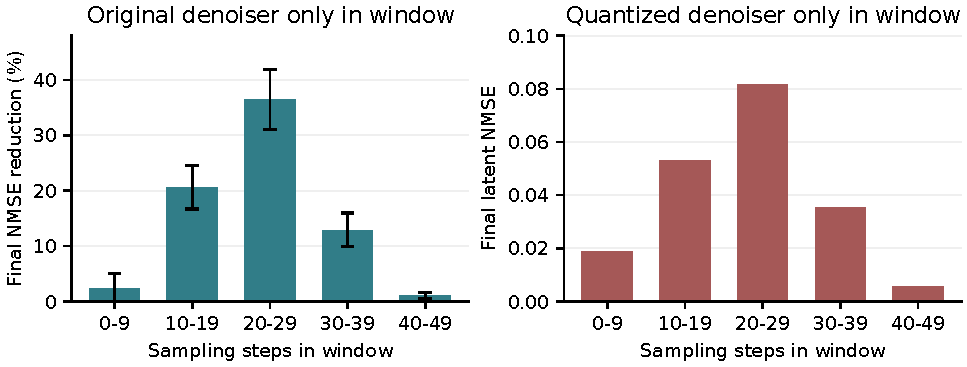
\includegraphics[width=\linewidth]{article_assets/temporal_windows.pdf}
 \caption{Temporal interventions on 256 paired trajectories. Left: reduction in final latent NMSE when the original denoiser is used only in the indicated window; error bars are paired bootstrap 95\% intervals. Right: final NMSE when quantization is used only in that window. Sampling-step indices are zero-based and increase as diffusion timesteps decrease. These hybrid trajectories require access to the original model and are diagnostic, not equal-bpp competitors.}
 \label{fig:windows}
\end{figure}

Both tests in Figure~\ref{fig:windows} identify steps 20--29 as the most consequential of the five equal-length windows. Restoring this interval reduces NMSE by \MiddleGainSmall\% (95\% interval \MiddleCILow--\MiddleCIHigh\%), while restoring steps 40--49 reduces it by only \LateGainSmall\%. An earlier, larger 1,000-pair experiment over three windows gives the same ordering: the middle-window improvement is \MiddleGainThousand\% (\MiddleLargeCILow--\MiddleLargeCIHigh\%). For this middle window, original diffusion timesteps run from 591 to 408. The result supports investigating middle-step sensitivity rather than selecting calibration weights solely by late error peaks. Effects across windows are nonlinear and cannot be added as independent shares of total error.

\subsection{Structural sensitivity}\label{sec:structural}

Restoring one family of original weight matrices and biases across all 28 blocks provides a second localization test. On 1,000 paired trajectories, adaLN restoration gives the largest reduction among the tested families (Table~\ref{tab:families}), even though MLP contains more matrix weights. The budgets are unequal, however, so this is not a ranking under equal memory or equal numbers of restored parameters.

\begin{table}[t]
 \centering
 \caption{Restoring one original layer family, with the rest of the denoiser quantized. All rows use 1,000 paired trajectories; the fully quantized control has NMSE \FamilyBaseline{}. Weight counts exclude biases.}
 \label{tab:families}
 \small
 \begin{tabular}{lrrrr}
  \toprule
  Family & Matrix weights (M) & Share of quantized weights & NMSE$\downarrow$ & Reduction \\
  \midrule
  \FamilyRows
  \bottomrule
 \end{tabular}
\end{table}

The adaLN modulation output consists of attention/MLP shifts, scales, and residual gates. In a follow-up on 256 paired trajectories, restoring just the MLP-gate rows reduces NMSE by \GateMLPGain\% (\GateMLPCILow--\GateMLPCIHigh\%), compared with \ShiftMLPGain\% for the MLP shift. Each of the six row groups contains 37,158,912 matrix weights, allowing an equal-size comparison within adaLN. These exploratory intervals do not include a multiple-comparison correction. An additional output-level test replaces the model's predicted noise or variance on its own current latent: original noise prediction removes more than 99.9\% of final NMSE, whereas original variance changes it by only about 0.12\%. This is an output oracle, not restoration of the already-unquantized final-layer weights. It supports prioritizing noise-prediction reconstruction in subsequent fitting experiments.

\subsection{First attempts at adaptation}\label{sec:refit}

We test whether a simple temporal modification can already convert the diagnostics into better FID. Starting from the transferred VQDM representation, we freeze indices, scales, and biases and update only codebook values using the teacher-statistics reconstruction objective. This is additional codebook fitting, distinct from the no-subsequent-fine-tuning baseline; it does not train dense model weights or use an end-to-end image loss.

The first study uses 200 Adam updates per layer and groups sampling steps as $[0,30)$, $[30,40)$, and $[40,50)$. We compare uniform weights $(1,1,1)$ against $(1,1,2)$ and $(1,2,2)$; the weights multiply the groups' second-moment contributions, rather than assigning equal total mass to differently sized groups. A second study fits separate codebook values for all three groups, sharing indices and scales. It uses 200 updates per group and therefore includes a single-codebook, 600-update control. The partition does not isolate the middle window identified above, so these experiments test naive late emphasis and coarse specialization, not every form of temporal adaptation.

\begin{table}[t]
 \centering
 \caption{Completed codebook-refitting studies; each variant is evaluated on 10,000 images. Controls are specific to each study. The final column gives the number of codebook updates per layer, summed across temporal sets.}
 \label{tab:refit}
 \small
 \begin{tabular}{lrrrrr}
  \toprule
  Variant & bpp & FID$\downarrow$ & sFID$\downarrow$ & IS$\uparrow$ & Updates \\
  \midrule
  \multicolumn{6}{l}{\emph{Temporal weighting}} \\
  \WeightedRows
  \midrule
  \multicolumn{6}{l}{\emph{Separate temporal codebooks}} \\
  \TemporalRows
  \bottomrule
 \end{tabular}
\end{table}

Uniform refitting yields lower FID than either late-emphasis variant (Table~\ref{tab:refit}). Three temporal codebook sets also fail to beat the 600-update uniform control while increasing storage by 4,587,520 bytes. These are small single-run differences, without repeated quantizer seeds or FID confidence intervals. Some continued evaluations span different GPU allocations, and their control values differ slightly from Table~\ref{tab:baseline}; we retain each study's own control rather than combining them. The evidence does not yet support a quality benefit from these simple temporal modifications.

\section{Discussion and Next Steps}\label{sec:disc}

The completed experiments establish a transfer gap and localize promising targets, but do not yet provide an improved quantizer. Middle-step interventions and adaLN restoration motivate testing middle-sensitive calibration and component-aware block/output reconstruction under an unchanged storage budget. The lack of improvement from naive late weighting is consistent with the intervention results; it does not rule out other temporal criteria. Likewise, restoring original weights only identifies sensitivity and cannot substitute for an equal-bpp compression experiment.

Further work should separate the effects of temporal weights, reconstruction level, code reassignment, and optimization budget, then validate selected variants with full image-generation metrics and independent calibration/quantizer seeds. Comparisons with published methods must control the quantized layers, activation precision, sampler, and evaluation sample count. Until those checks are completed, the strongest supported conclusion is diagnostic: a static layerwise objective transfers imperfectly, and the importance of a denoising error cannot be inferred from its timestep magnitude alone.

\bibliographystyle{unsrtnat}
\bibliography{references}

\end{document}
